\documentclass[11pt,a4paper,landscape]{article}
\usepackage[utf8]{inputenc}
\usepackage[english]{babel}
\usepackage{amsmath}
\usepackage{cite}
\usepackage{amsfonts}
\usepackage{amssymb}
\usepackage{makeidx}
\usepackage{graphicx}
\usepackage{tikz}
\usepackage{listings}
\usepackage{hyperref}
\author{jacmalm@kth.se}
\title{DD2343 Assignment 1}
\begin{document}

\maketitle
\newpage
\section{Principal Component Analysis}

\subsection{Explain why data-centering is required before performing PCA.  What might happen if we perform PCA on non-centered data?}
\label{mean-center}

PCA attempts to find new axes that are linear combinations of the old axes, such that these new axes, or principal components, minimize the mean squared distance between the original data points and their projection onto the principal axes \cite{pca_lecture_book}.  One key thing to note is that these principal components are limited by the need to cross through the origin. This limitation means that data that is shifted cannot be approximated as well. A simple example is to consider the points $\lbrace-1, 1\rbrace$, $\lbrace0,0,\rbrace$, $\lbrace1, -1\rbrace$. These points all lie perfectly along a 1 dimensional manifold, the line with slope -1 going through the origin. The mean of this dataset is 0. Thus, we expect the first principle component to consist of this line, and we expect all of the variance to be explained by the first principle component, as the PCA model is perfectly respected.When we run the PCA code (with the lines responsible for centering the data commented out in the SKLearn library file) given in appendix 1, this is exactly what we see. Great! PCA works.\newline

However, if we shift the location of this manifold, while keeping its shape intact, this will change. If we now consider the points $\lbrace49, 51\rbrace$, $\lbrace50,50\rbrace$, $\lbrace51, 49\rbrace$, it is easy to see that they also perfectly lie along a line, indeed a line with the same slope as the previous example. However, this line does not pass through the origin, and will thus not be found by PCA. Instead, what we expect to happen, is that the first principle component will be a line that goes through the origin and minimizes the distance from the data points and their projection onto the first principle axis. As the data is symmetric around their mean, we expect this to be a line going through the mean point,$\lbrace50,50\rbrace$, and the origin.This is a line with slope 1. In fact, this line is perpendicular to the line that the data points lie along. When looking at the explained variance, we can also see that this line does not explain all of the variance, necessitating us to use both principal components to perfectly be able to get back all of our data, meaning that PCA fails to detect the inherent 1-dimensionality of the dataset. Again, these conclusions are verifiable with provided code in Appendix 1, and visually demonstrated in figure 1 and figure 2.

\includegraphics[width=\textwidth]{figure1_2.pdf}

\subsection{Is a single SVD operation sufficient to performing PCA on both the rows and columns of a data matrix}
\label{svd}

The first step we do when we perform PCA is to mean center the data. In \ref{mean-center} we showed why this was necessary. However, when we mean center, we only mean center along one of the two axes. If columns represent a feature and rows represent observations, we can view each column as containing observations of a distinct random variable. Thus in this case, mean centering along each column is interpreted as shifting the mean of the distribution responsible for generating this column to zero. This keeps the structure of the data intact.\newline

When we wish to perform PCA on the transpose of our data matrix, the interpretation of the rows and axes switch. Furthermore, our data will not be mean centered after transposing the matrix, as in the previous PCA operation we only center along the columns.\newline

We are not able to mean center along rows and columns before performing both PCA operations, as this will alter the distribution of our data set. Imagine a case where we are given a data matrix with $ n $ observations and two normally distributed features, $x, y$. Each one of these observations can be plotted on a 2d plane, where its position on the x-axis is given by its value of feature $ x $ and its y-value is given by value of feature $ y $. If we presume that these features are independent, our data points will fill in a circle as $ n \rightarrow  \infty $. Centering along each column will shift the center of this circle to the origin. Centering along the rows means that we need each observation to fulfill the following equation
$$ 0 = \frac{1}{2} (x_{i} + y_{i},) i \in \lbrace 1 ...  n\rbrace $$

We can easily see that this will force all points to lie on the line $ y =  -x $, drastically changing the distribution of our observations.\newline

Thus, we cannot perform PCA on both the rows and columns with one SVD operation as we need to mean center the matrix before the SVD operation and after the transposition.

\subsection{Explain why the use of the pseudo-inverse is a good choice to obtain the inverse mapping of the linear map}

The pseudo-inverse is a good choice to obtain the inverse mapping because when the PCA model is fully respected, that is our data points $\textbf{y} \in \mathbb{R}^d$ are fully contained within a subspace $\textbf{U} \in \mathbb{R}^k$ where $k < d$, and \textbf{U} is the column space of \textbf{W}, $\textbf{W}^{+}$ is the inverse mapping of \textbf{W}, even when \textbf{W} is non-square.\newline

However, when the PCA model is not fully respected and there are points in \textbf{y} that lie outside of \textbf{U}, the pseudo-inverse computes the inverse mapping from the points projected onto \textbf{U}, which is the approximation that minimizes the euclidean distance between computed and actual points\cite{pseudoinverse}.\newline

Thus, using the pseudo-inverse of the linear transformation that is hypothesized to have generated \textbf{y} from \textbf{x}, allows us to compute the projection onto the PCA axes even for points that do not completely lie within the $k$ dimensional column space, which often occurs due to noisy measurements or an underlying model not quite aligned with the PCA assumptions.

\subsection{Derive PCA using the criterion of variance maximization and show that you get the same results as with the criterion of minimizing the reconstruction error}

We begin by assuming that our data set are observations from a set of \textit{d} jointly distributed gaussian variables, \textbf{Y}, that have undergone a linear transformation \textbf{W} applied to a set of \textit{p} latent variables \textbf{X}, where $p < d$. This linear transformation is restricted to be an axis change, meaning that \textbf{W} is orthogonal.\newline

We assume that the latent variables \textbf{x} are uncorrelated. This means that the covariances are zero, and that the covariance matrix $C_{x} $ is diagonal.

The covariance of \textbf{x} is given by

$$ C_{x} = \mathbb{E}[xx^{T}] $$

Similarly, the covariance of y is given by 
$$ C_{y} = \mathbb{E}[yy^{T}] $$

Rewriting this equation using the PCA assumptions ($y = Wx$)

$$ C_{y} = \mathbb{E}[Wxx^{T}W^{T}] $$

Using the fact that expectation is a linear operator

$$ C_{y} = W\mathbb{E}[xx^{T}]W^{T}$$
$$ C_{y} = WC_{x}W^{T}$$

Since \textbf{W} is orthonormal

$$ W^{T}C_{y} = W^{T}WC_{x}W^{T}$$
$$ W^{T}C_{y}W = W^{T}WC_{x}W^{T}W$$
$$ W^{T}C_{y}W = IC_{x}I$$
$$ W^{T}C_{y}W = C_{x}$$

Since $ C_{y} $ is symmetrical we can use its spectral decomposition to rewrite it as
$$ C_{y} = Q\Lambda Q^{T} $$

And thus
$$C_{x} = W^{T}Q\Lambda Q^{T}W$$

Remembering our assumption that the variables in \textbf{x} are uncorrelated,  $C_{x}$ is a diagonal matrix. Since $\Lambda$ is diagonal and $Q$ is orthogonal, 
$$WQ^{T} = I$$
$$WQ^{T}Q=QI$$
$$W= Q$$

and

$$ C_{x} = \Lambda $$

However, since $C_{X}$ is a $p\times p$ matrix only the first $p$ eigenvalues of $\Lambda$ are non-zero (assuming the PCA model is followed). Thus the above equality only holds when choosing the $p$ first eigenvectors when sorting by corresponding eigenvalue size, and restricting $\Lambda$ to its non-zero diagonal values. \newline

This suggests that the eigenvalues of the spectral decomposition of $C_{y}$ represent the amount of variance captured in the direction of its corresponding eigenvector, with our eigenvectors spanning the linear subspace that contains \textbf{y}. Thus our principal axes are given by $Q$ in order of importance, when $\Lambda$ is sorted in descending order \cite{book}.\newline

Similarly, when deriving PCA from a minimization of squared error perspective, our principal components are given by \textbf{U}, with $X = U\Sigma V^{T}$. As shown in \ref{svd}, $U = Q$, and $\Sigma^2$ is proportional to $\Lambda$. Thus, due to the monotonicity of the square function, the principal axes will appear in the same order, and have the same values. As our principal axes determine our PCA projection, we can conclude that the two derivations yield equivalent results\cite{book}.



\section{Multidimensional Scaling and Isomap}

\subsection{Explain intuitively why the double centering trick is needed to be able to solve for S given D}

Given a squared distance matrix \textbf{D} we wish to find Gram matrix \textbf{S}. As mentioned, the equation for this conversion is given by

$$ s_{ij} = -\frac{1}{2}(d^{2}_{ij} - s_{ii} - s_{jj})$$

The issue here is that we do not know the coordinates of our data points and as a result $s_{ii}, s_{jj}$ are unknown, making this definition circular. When we assume that our data is mean centered (which we are allowed to do since distance is invariant to location), it can be shown that

$$ -(s_{ii} + s_{jj}) = \mu_{ij} - \mu_{i} - \mu_{j} $$

These $\mu$'s refer to the means of the distance matrix we are given. Thus, by assuming that our data is centered, we can rewrite the unknowns in our conversion equation in terms of information contained in the distance matrix that we are given. This makes the conversion possible \cite{book}.

The double centering trick simply performs $$ s_{ij} = -\frac{1}{2}(d^{2}_{ij} +( \mu_{ij} - \mu_{i} - \mu_{j}))$$ for all matrix elements in \textbf{D}, converting our given distance matrix into the desired Gram matrix.


\subsection{Use the same reasoning as in the previous question to argue that $s_{ij}$ can be computed as $s_{ij} = -\frac{1}{2}(d_{ij}^{2} - d_{1i}^{2} - d_{1j}^{2})$}

Comparing the original equation
$$ s_{ij} = -\frac{1}{2}(d^{2}_{ij} - s_{ii} - s_{jj})$$
with
$$s_{ij} = -\frac{1}{2}(d_{ij}^{2} - d_{1i}^{2} - d_{1j}^{2})$$

We can deduce that
$$s_{ii} + s_{jj} = d_{1i}^{2} + d_{1j}^{2}$$
must hold.\newline

From Lee and Verleysen \cite{book} equation 4.42 we know that we can rewrite this equation accordingly
$$ s_{ii} + s_{jj} = (\langle \mathbf{y_{1}} \cdot \mathbf{y_{1}} \rangle - 2\langle \mathbf{y_{1}} \cdot \mathbf{y_{i}} \rangle + \langle \mathbf{y_{i}} \cdot \mathbf{y_{i}} \rangle) + (\langle \mathbf{y_{1}} \cdot \mathbf{y_{1}} \rangle - 2\langle \mathbf{y_{1}} \cdot \mathbf{y_{j}} \rangle + \langle \mathbf{y_{j}} \cdot \mathbf{y_{j}} \rangle)$$

Where $\mathbf{y_{1}}$ represents the vector holding the coordinates of the first point. Now, if instead of assuming that our data points are mean centered and assume that the first data point is located on the origin, which we are allowed to do since this does not affect the distance between any of the points, the above equation reduces to

$$ s_{ii} + s_{jj} = \langle \mathbf{y_{j}} \cdot \mathbf{y_{j}} \rangle + \langle \mathbf{y_{i}} \cdot \mathbf{y_{i}} \rangle$$
$$ s_{ii} + s_{jj} = s_{ii} + s_{jj} $$

Thus we can see that we are justified in using this alternate equation to calculate our Gram matrix. It will not result in the same mapping as if we used $ s_{ij} = -\frac{1}{2}(d^{2}_{ij} +( \mu_{ij} - \mu_{i} - \mu_{j}))$, which will be mean centered, whereas our equation will fix the location of the first data point to the origin.


\subsection{Argue that the process to obtain the neighbourhood graph G in the Isomap method may yield a disconnected graph.  Provide an example.  Explain why this is problematic.}

The Isomap algorithm works similarly to MDS in that it relies on computing a Gram matrix \textbf{S} from a distance matrix \textbf{D}. However, dissimilarly to MDS, this distance matrix is not made up of euclidean distances. Instead, the distances are approximations of the shortest path from point A to point B where the path is restricted to the theoretical manifold our data distribution makes up. Computing the shape of this manifold as well as the length of the path through the manifold from point A to B is infeasible. An approximation of the manifold can be created by drawing a neighbourhood graph G. This neighbourhood graph G is created one of two ways. Either by joining each point to its \textit{k} nearest neighbours, where a point A is considered closer to point B than to C if the euclidean distance between A-B is smaller than A-C.  Alternatively the neighbourhood graph can be constructed by choosing to join a point A to all of its neighbours that lie within a certain distance \textit{d}.\newline


To demonstrate how this process can lead to a disconnected graph,  assume we have the following nodes located at given coordinates.

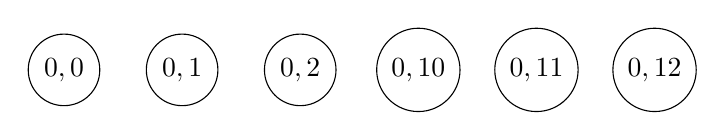
\begin{tikzpicture}[node distance=15mm, main/.style = {draw, circle}] 
\node[main] (1) {$0,0$};
\node[main] (2)[right of = 1] {$0,1$};
\node[main] (3)[right of = 2] {$0,2$};
\node[main] (4)[right of = 3] {$0,10$};
\node[main] (5)[right of = 4] {$0,11$};
\node[main] (6)[right of = 5] {$0,12$};

\end{tikzpicture}

If we go by the k-nearest neighbour approach and set k=2, or go by max euclidean distance between nodes and set \textit{d} to smaller than 8, our resulting graph will be disconnected.

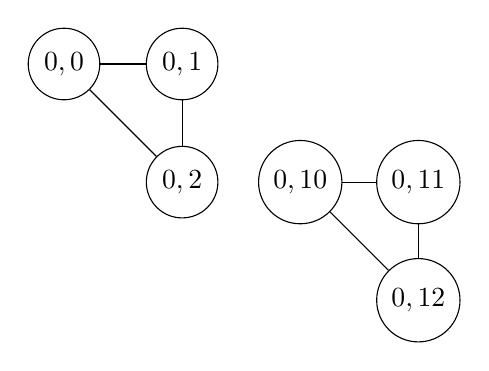
\begin{tikzpicture}[node distance=15mm, main/.style = {draw, circle}] 
\node[main] (1) {$0,0$};
\node[main] (2)[right of = 1] {$0,1$};
\node[main] (3)[below of = 2] {$0,2$};
\node[main] (4)[right of = 3] {$0,10$};
\node[main] (5)[right of = 4] {$0,11$};
\node[main] (6)[below of = 5] {$0,12$};
\draw(1) -- (2);
\draw(2) -- (3);
\draw(3) -- (1);
\draw(4) -- (5);
\draw(5) -- (6);
\draw(6) -- (4);
\end{tikzpicture}

According to the Isomap algorithm, when we compute the distance matrix, the entry between point A and point B will be the summation of the distances between all nodes that lie along the shortest path between A and B through the neighbourhood graph G constructed in the previous step. If this is a disconnected graph, the distance between any point A to any point B where A and B are members of different disjoint subsets in G will be infinite, or undefined. In either of these cases the spectral decomposition of the Gram matrix corresponding to the distance matrix will be undefined and the Isomap algorithm will fail.


\section{Programming task}

\subsection{Data collection}
I collected a list of all the worlds capital cities from \url{https://github.com/icyrockcom/country-capitals/blob/master/data/country-list.csv}.

\bibliography{mybib}
\bibliographystyle{plain}

\section{Appendices}
\subsection{Appendix 1}
\lstinputlisting[language=python]{../code/centering_pca.py}
\end{document}